\epigraph{``The grandest discoveries of science have been but the rewards of
    accurate measurement and patient long-continued labour in the minute
sifting of numerical results.''}{William Thompson, \nth{1} Baron Kelvin}

\section{Models of the Atomic Nucleus: Overview}
The nuclear many-body problem remains one of the most challenging problems in
physical science despite a century of experimental and theoretical advances.
Basic questions, including how nucleons are distributed throughout the nuclear
volume and how they share the energy of binding, are still only qualitatively
answered. At the core of the issue is the short-range and extremely strong
nature of nuclear forces, which confine
quarks to nucleons and cannot be treated perturbatively in the MeV-energy regime of
nuclear physics. Rather than take a truly ab-initio approach where quarks and gluons
are the relevant degrees of freedom, a series of approximations must be made
for calculations to be tractable. As long as the energy domain is less than that
of the lowest-lying nucleon excitation, it is well-justified to reduce the
nuclear problem to choosing protons and neutrons as the nuclear building blocks.
The proton and neutron masses are so close, and their behaviors in the nucleus so similar,
that the problem can be further simplified by introducing a new (approximate) quantum number
I, the isospin, and treating protons and neutrons as generic "nucleons" with differing I.

Starting with these simplifications, many nuclear models have been developed to describe existing 
data on nucleon-nucleon, nuclear-nuclear, lepton-nuclear scattering as well as
nuclear binding. Successful models should not only reproduce existing
experimental data accurately but also posses predictive power for as-yet unmeasured
experimental data. For parametric models
with many tunable parameters, these two criteria pull in oppositive directions:
increasing the number
and acceptable range of model parameters often helps to reproduce experimental data but may
jeopardize predictive power if new parameters are not connected to the underlying physics.
I begin by presenting a few workhorse model families most relevant
to this dissertation and omit many others (notably, Density Functional Theory
and Lattice QCD). Each model's successes,
failures, and regimes of validity are briefly discussed, with extra attention paid
to each model's confrontation with certain challenging data.
A central motivation for this work is to provide experimental data most useful
for a particular type of optical model of the nucleus that attempts to
connect nuclear structure information (i.e., bound state information) with nuclear
reactions, a longtime goal in nuclear physics. 

\subsection{Liquid Drop Model}

The Liquid Drop Model (LDM) describes nuclei as drops of ideal nuclear fluid and
has been successfully employed since the earliest days of nuclear science to
describe nuclear masses and other ground-state properties. The binding of each
nucleus is approximated by five physically-intuitive terms appropriate for
a droplet of nuclear matter:

\begin{equation} \label{LDM}
    BE(Z, N) = Vol + Surface + Coulomb + Asymmetry + Pairing
\end{equation}

a volume term that describes "bulk" binding that would be experienced in an
infinite sea of nuclear matter

a surface term that incorporates the finite size of a nucleus (i.e., it is a
drop, not an ocean), equivalent to considering surface tension,

a coulomb term that incorporates the electric repulsion experienced by protons
kept in close proximity inside the drop,

an asymmetry term representing the relative chemical potential of neutrons and
protons as a function of their relative population (which can be re-balanced by
beta decay),

a pairing term to account for the experimental observation that nuclei with an
even number of both protons and neutrons are slightly more bound, implying a
favorable pairing interaction

The free parameters in each term can be fitted to the hundreds of well-measured nuclear masses
across the chart of nuclides. These five simple terms are quite successful
in describing masses and radii of spherical nuclei, leading early nuclear
scientists to expect that shell structure was less important in the nuclear
many-body problem than in the atomic one. In this ansatz, the quantum
nature of constituent nucleons is completely ignored, so the LDM is  
unsuitable for extracting wavefunction information or predicting scattering
cross sections.

The Droplet Model \cite{MyersAndSwiatecki} considers a systematic two-dimensional expansion of
Eq. \ref{LDM} about two fundamental independent quantities, the nucleon density
and neutron-proton asymmetry:

\begin{equation}
    \epsilon = -\frac{1}{3}\frac{(\rho - \rho_{0})}{\rho_{0}}
\end{equation}

\begin{equation}
    \delta = \frac{\rho_{n}-\rho{z}}{\rho}
\end{equation}

\noindent
In the above, $\rho_{0}$ is the saturation density of 0.16 nucleons fm$^{-3}$. Relevant quantum
effects, such as changes in level densities near shell closures
that affect the observed masses, can be incorporated through a series of corrections
that approximate shell effects and geometric deformation.
The Droplet Model of Atomic Nuclei deploys 9 
independent coefficients to describe spherical droplets and 6 additional
coefficients to accommodate non-spherical effects. This expanded scope
can successfully recover the degree of ground state deformation in non-spherical
nuclei and fission barriers.

Because the LDM is not based upon shell structure, its utility has diminished
compared to other models that reproduce additional experimental data collected
over the last fifty years. However, the model still is a useful reference for providing 
information about bulk properties of nuclear matter. For example, by the 1980s,
it was clear that the isotope shift in the nuclear RMS
charge radii, shown for the even-A Sn isotopes in Fig.
\ref{SnIsotopeShift} \cite{Anselment1986},
is critically connected to difference in RMS radius 
between the neutron and proton distributions, commonly referred to as the
"neutron skin" \cite{Otten1989}.
In a Droplet Model picture, the slope of the isotope shift is linked to the symmetry energy $J$, 
density dependence of the symmetry energy
$L$, and surface stiffness coefficient $Q$, the same bulk quantities that determine
neutron skin thickness \cite{Myers1969, MyersAndSwiatecki, Berdichevsky1988}.
Without addition experimental constraints, the $J$, $L$, and $Q$ parameters form an
underdetermined system from which unique values cannot be recovered, even if the
consensus value of $J \approx$ 30 MeV is used to reduce the parameter space.
As was already pointed out 50 years ago by Myers \cite{Myers1969},
the single-particle configuration of a given nucleus may have a significant
effect on the formation and size of such a skin.

\begin{figure}
    \centering
    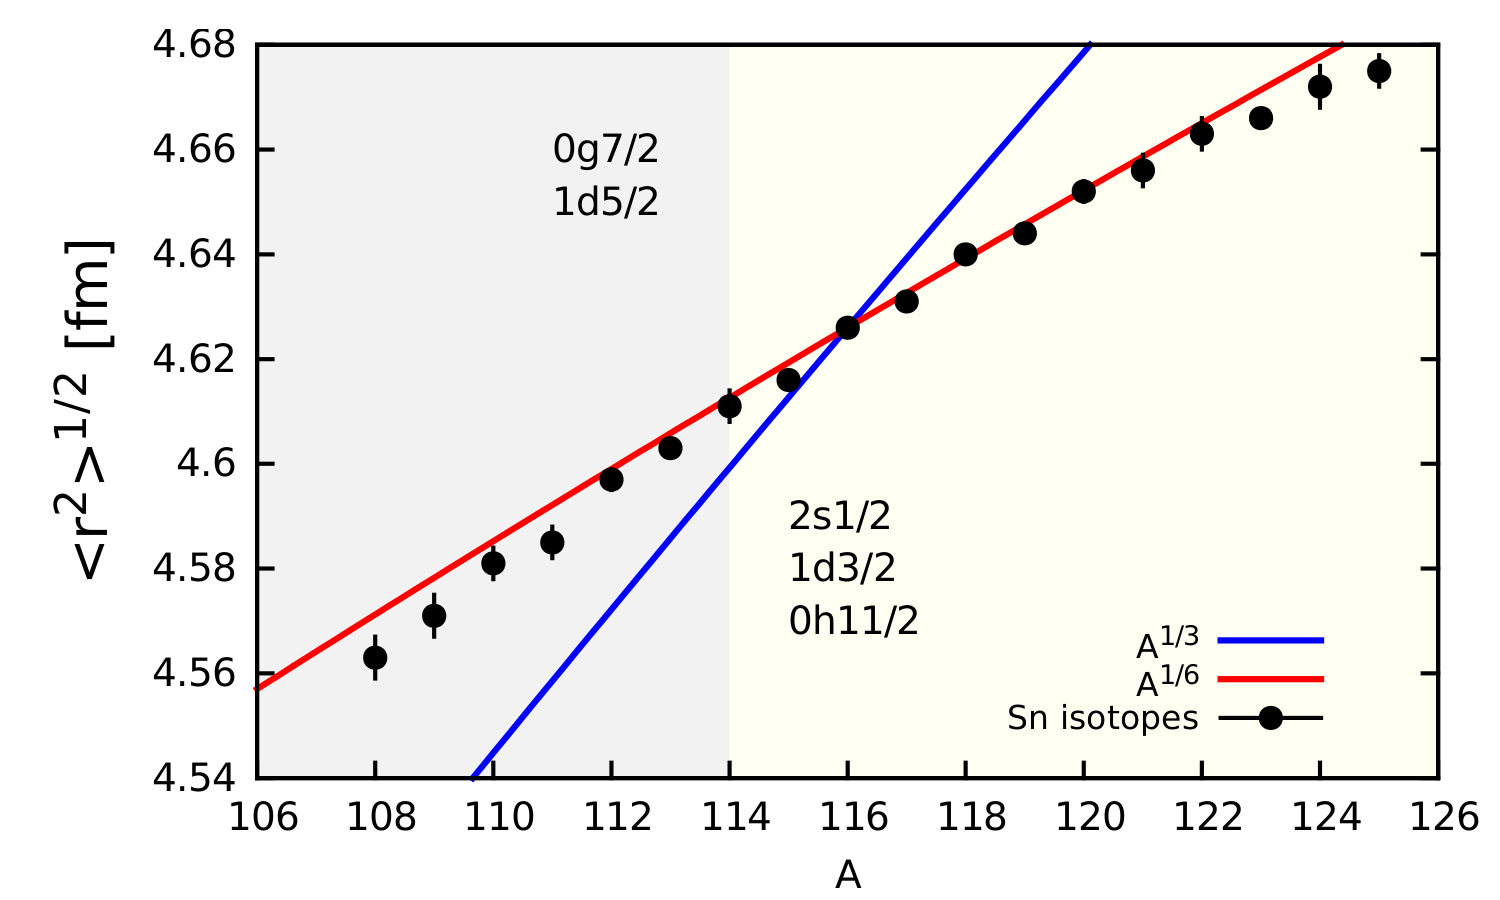
\includegraphics[width=0.8\textwidth]{figures/SnIsotopeRMSRadii.png}
    \caption{RMS charge radii in Sn nuclei display a nearly-linear isotope
    shift. The A=106-114 region and A=114-116 region are shaded and labeled
    indicating the expected single-particle occupation of the valence neutrons.
    An isoscalar treatment that only accounts for size scaling predicts an
    A$^{\frac{1}{3}}$ slope as neutrons are added, but the data show an
A$^{\frac{1}{6}}$ slope instead, which is connected to the symmetry energy
and its density-dependence. Data from Anselment et al. \cite{Anselment1986}}
    \label{SnIsotopeShift}
\end{figure}

\subsection{Mean-field models}
Mean field models begin with a simple motivation: that nucleons
traverse the nuclear environment independently, in an average
potential generated by all other nucleons, smeared out over nuclear volume.
The assumption of independent nucleon motion may seem dubious, given the
crowded environment of the nucleus and immense strength of nucleon-nucleon forces,
but the Pauli exclusion principle provides some justification.
From such a mean field, a shell model can be developed wherein nucleons obey a nuclear aufbau, 
filling orthogonal states with quantum numbers N, L, and J, as electrons do in the atomic 
case, resulting in shell structure. From a mean field consisting of a central
potential and a spin-orbit potential, as in the seminal shell-model work of Goeppert-Mayer
and Jensen \cite{GoeppertMayer1955}, the basic ground-state quantum properties of most nuclei
(spins, parities, magnetic moments) are recovered. In addition, nucleons can be
excited into higher (but still bound) states and the low-lying excitation
spectra predicted. The consequences of shell structure are obvious
in the experimental record, including increased particle separation 
energies and decreased nuclear radii at shell closures, directly analagous to
the atomic ionization energies and radii in the noble gases. The independent
treatment of nucleons is most valid near shell closures,
where the level density is reduced, and near beta-stability, where coupling to
the asymptotically-free states of the continuum is least important.

In a modern mean-field approach, the central average potential is considered
only as a starting point for a perturbative
expansion that collects residual nucleon-nucleon interactions associated with
correlated behavior, most of which can be categorized as collective rotations
and vibrations. Coupled excitations of
two or more nucleons to higher orbitals within or across shells and relativistic effects may 
be included to accommodate the experimental phenomena under investigation.
In light systems, where the number of nucleons is not too large, every nucleon
may be allowed to participate in excitations into the valence space of the model
(a ``no-core shell model"). As the system size increases, the configuration space grows
combinatorially until calculations become prohibitively expensive for a no-core
shell model approach. To ease calculations for these nuclei, a variety of approaches
are employed, including simply restricting the valence space and prohibiting deeply-bound 
nucleons from participating in excitations, hopefully while still capturing the
essense of the physical property under investigation. In very light nuclear
systems (A$<$12), the underpinning
mean field assumption begins to break down as nucleons become too granular to treat on average.

%\begin{figure}
%    \includegraphics[width=0.8\textwidth]{figures/ShellModel.png}
%    \caption{Nuclear shell model }
%    \label{ShellModel}
%\end{figure}

Beyond-mean-field approaches dispense with the assumption of an average
potential and build up nuclear Hamiltonian from nucleon-nucleon potentials
folded over the nucleon density profile. An advantage
of this approach is the connection between fundamental nucleon data
(for example, neutron-proton scattering phase shifts) and the many-body
properties of light nuclear systems \cite{AV18}. Many studies have
confirmed the importance of spin-orbit, isospin, tensor, and three-body terms
in the nucleon-nucleon potential for accurately reproducing structure in even
very light nuclei. 

- Connect to chiral effective field theory work for calculating optical potentials
and examining isovector component of potential, especially w/r/t to exotic
nuclei near driplines. Nucleons are still degree of freedom, but allowed to exchange effective 
pions that include the quark-quark interactions that comprise the strong nuclear force.
- computational limitations to beyond-mean-field above A=12?

In contrast to the LDM, both mean-field and beyond-mean-field models have
something to say about nuclear reactions and decays. Incident nucleons or nuclei can
transfer nucleons to/from the nucleus being modeled and standard
techniques of scattering theory can be applied, though at high excitation
energies and where the continuum becomes important, accuracy declines.

Investigations sensitive to the deeply-bound nucleons reveal some cracks in the mean-field
picture.  (e,e'p) measurements \cite{eep1, eep2} and high-energy (p,2p) knockout reactions 
\cite{knockout1, knockout2} show a depletion of occupancy from ~10\% (near the Fermi surface) to
over 30\% (in deeply bound orbitals), contrary to the mean-field assumption of
full nucleon occupancy of all levels below the Fermi surface. In quasi-free
scattering experiments, deeply-bound nucleons are seen to occupy a broad range
of possible energies, challenging the assumption that each
nucleon resides a single subshell with a discrete energy. Additionally, when mean-field
potentials are used to generate charge-density distributions, as measured in
elastic electron scattering experiments \cite{DeVries1987}, the nuclear core is found to
have too high a charge density \cite{ChargeDensityCoreExample}. Similar
effects have been seen in GeV-scale deep-inelastic scattering that probes the momentum
distribution of quarks in deeply-bound nucleons. Excess high-momentum content is
found in the tails of the momentum distribution, indicating that a few percent of the time, 
nucleons are traveling far faster than expected. Short-range correlations, or
interactions between quarks of different nucleons that are in close proximity,
are invoked to explain these differences.
Quantitatively explanation of these issues continues to be an outstanding issue in nuclear 
theory and motivates improved data-driven descriptions of behavior deep in the nucleus.
These results also raise questions about
the when nucleons can be assumed to be good degrees of freedom and quark degrees of freedom 
can be ignored.

\subsection{Optical Models}
For the LDM and mean-field models presented thus far, the primary motivation has been recovery
of structural observables like nuclear masses, radii, low-lying excitations, and magnetic moments. 
A comprehensive understanding of the nucleus must also say something about what
nuclei \textit{do}, as in higher-energy nucleon-nucleus scattering experiments
and in astrophysical reactions.
The nuclear optical model (OM) was developed to this end and continues to be an
widely-used tool for generating nucleon, $\alpha$, and heavy-ion scattering
cross sections, though it has had less to say about nuclear structure. Basic
motivations for OMs, plus references to successful OM potential parameterizations,
are summarized here.

Due to the magnitude of the strong nuclear force, it might be expected that 
the interaction of an incident neutron on a nucleus should be strongly
absorptive, with only a small contribution from elastic scattering. Thus, the
earliest model for neutron scattering describes the nucleus as a constant-density
sphere that interacts strongly with incident neutrons approaching within a nuclear radius
\cite{Feshbach1949}. In this ``strongly-absorbing sphere" (SAS) picture devoid of nuclear structure
or shell effects, \tot\ depends only on size scaling of the interacting bodies:
\begin{equation} \label{SASAbsolute}
    \sigma_{tot}(E) = 2\pi(R + \lambdabar)^{2}
\end{equation}
where $R=r_{0}A^{\frac{1}{3}}$ and $\lambdabar$ is the reduced de Broglie wavelength
of the incident neutron in the center of mass \cite{Fernbach1949, Satchler1980}. 

As neutron scattering experiments expanded to higher energies in the 1950s, 
neutron total cross section data emerged that challenged this picture. The total
cross section, \tot, is simply the sum of elastic and inelastic cross sections.
Due to the infinite range of the Coulomb force, \tot\ cross section is sensible only for
uncharged particles. In Fig.
\ref{SASphereVsExperiment}, neutron \tot\ data are shown from 2-500
MeV for nuclides from A=12 to A=208 \cite{Finlay1993, Schwartz1974, Poenitz1983, Abfalterer2000, 
Abfalterer2001}. Predictions for \tot\ given by Eq. \ref{SASAbsolute} are shown as thin dashed 
lines for each nucleus. Regular oscillations about the SAS model are clearly
visible, as is the trend for the oscillation maxima and minima to shift to \textit{higher}
energies as 
A is increased. At low energies, resonance structures are visible especially for light nuclides 
where the density of states is smallest. Note that at higher neutron energies, the experimental
cross sections drop below those predicted by the SAS model, illustrating
a increase in nuclear transparency.

\begin{figure}
    \centering
    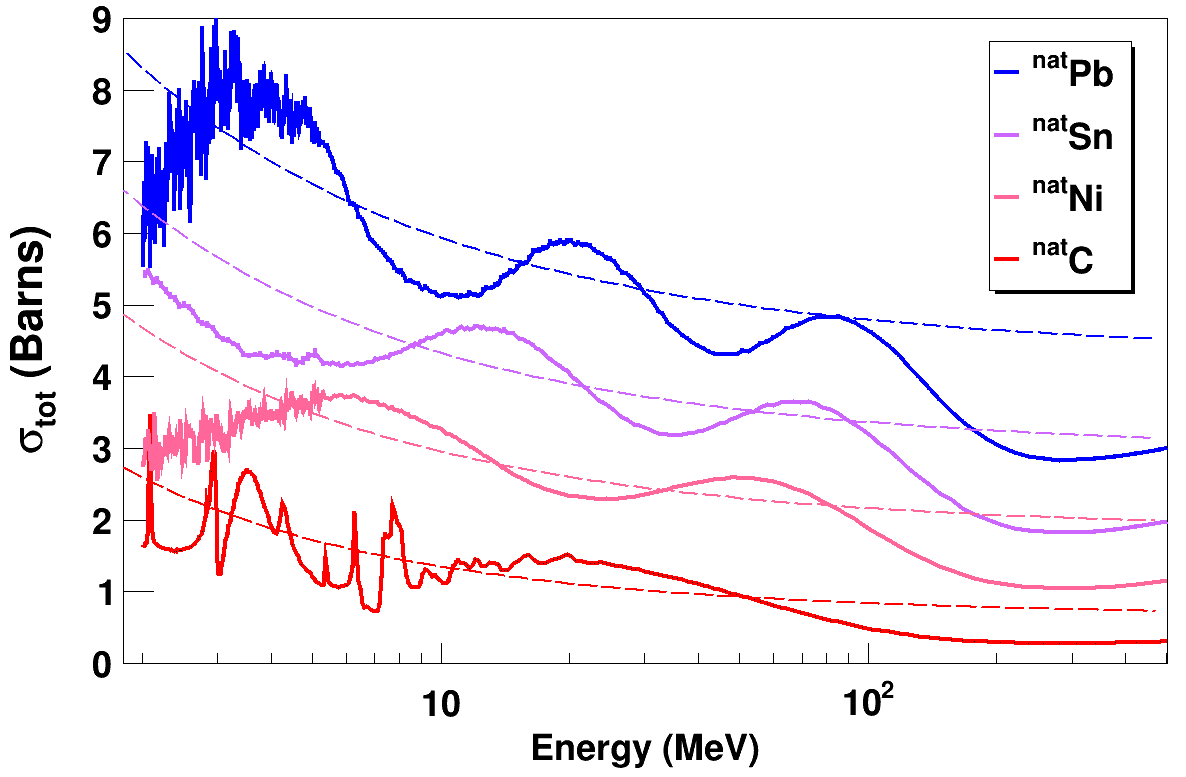
\includegraphics[width=0.8\textwidth]{figures/SASphereVsExperiment.png}
    \caption[Experimental neutron \tot\ data and strongly-absorbing-sphere predictions]
    {
        Experimental neutron \tot\ data on several natural samples (solid lines)
        from 2-500 MeV. The predictions of the crude strongly-absorbing-sphere
        model (Eq. \ref{SASAbsolute}) are shown as dashed lines. Resonance structures are
        clearly visible in the \cNat neutron \tot\ below 20 MeV.
    }
    \label{SASphereVsExperiment}
\end{figure}

These hallmark oscillations in the neutron \tot\ can be explained as the result
of a phase shift between 
neutron waves passing around the nucleus (unshifted) and waves passing
through the the nucleus, where they experience refraction
(illustrated in Fig. \ref{RamsauerPhaseShiftFigure}). This explanation was termed the ``nuclear 
Ramsauer effect" by Peterson \cite{Peterson1962}, based on the analagous effect seen in 
electron scattering on noble gases.

Following Angeli \cite{Angeli1970}, these considerations can be incorporated by
imbuing the strongly-absorbing sphere relations (equation \ref{SASAbsolute}) with an additional sinusoidal term:
\begin{equation} \label{OscillatoryModel}
    \tot = 2\pi (R+\lambdabar)^{2}[1 - \rho \cos(\delta)]
\end{equation}
where $\rho = e^{-\operatorname{Im}(\Delta)}$, and $\delta =
\operatorname{Re}(\Delta)$, with $\Delta$ the phase difference between the wave traveling
around and traveling through the nucleus. Thus, the amplitude of the oscillations provides the 
inelastic phase shift and the period of oscillation provides the elastic phase shift.
As can be seen from Eq. \ref{OscillatoryModel}, the large magnitude of the oscillations means that 
inelastic scattering (from $\operatorname{Im}(\Delta)$) accounts for only a small fraction of the 
total cross section, in turn implying a much larger mean free path for neutrons through the nucleus 
than would be expected in the absence of Pauli blocking \cite{Mohr1955}.

If the nucleus presents a spherical potential of radius $R$ and depth $U$, the total phase shift $\delta$ is:
\begin{equation} \label{phaseShift}
    \delta =
    \frac{\overline{C}\left(\left[{\frac{E+U}{E}}\right]^{\frac{1}{2}}-1\right)}{\lambdabar}
\end{equation}
where $\overline{C} = \frac{4}{3}R$ is the average chord length through the
sphere \cite{Angeli1970}. Rearranging Eq. \ref{phaseShift} in terms of A and E and
discarding leading constants yields:
\begin{equation}
    \delta \propto A^{\frac{1}{3}}\times\left(\sqrt{E+U}-\sqrt{E}\right)
\end{equation}
This form reveals an important relation: as A is increased, to maintain constant 
phase $\delta$, E must also increase \cite{Satchler1980, Peterson1962}. 
This is contrary to a typical resonance condition where an integer number of wavelengths
are fit inside a potential; in that case, to maintain constant phase as A is increased,
E must be decreased. Thus these \tot\ oscillations have been referred to as
``anti-resonances" or ``echoes" \cite{Satchler1980, McVoy1967}.

A new type of nuclear model is thus at hand: by replacing the intractable many-body problem
of the target nucleus by a complex, refractive potential, both elastic scattering (from the real 
part of the potential) and inelastic scattering (from the imaginary part) can be neatly 
explained. The existing mathematical machinery for calculating scattering of light from
refractive materials can then be repurposed for nuclear scattering, giving birth to
the ``optical model" of the nucleus \cite{Feshbach1958, McVoy1967}. In
practice, the potential is typically parameterized with a series of
terms centered on the nuclear surface and nuclear volume,
corresponding to differing physics thought to be important for these areas (much
as in the Droplet Model).

\begin{figure}
    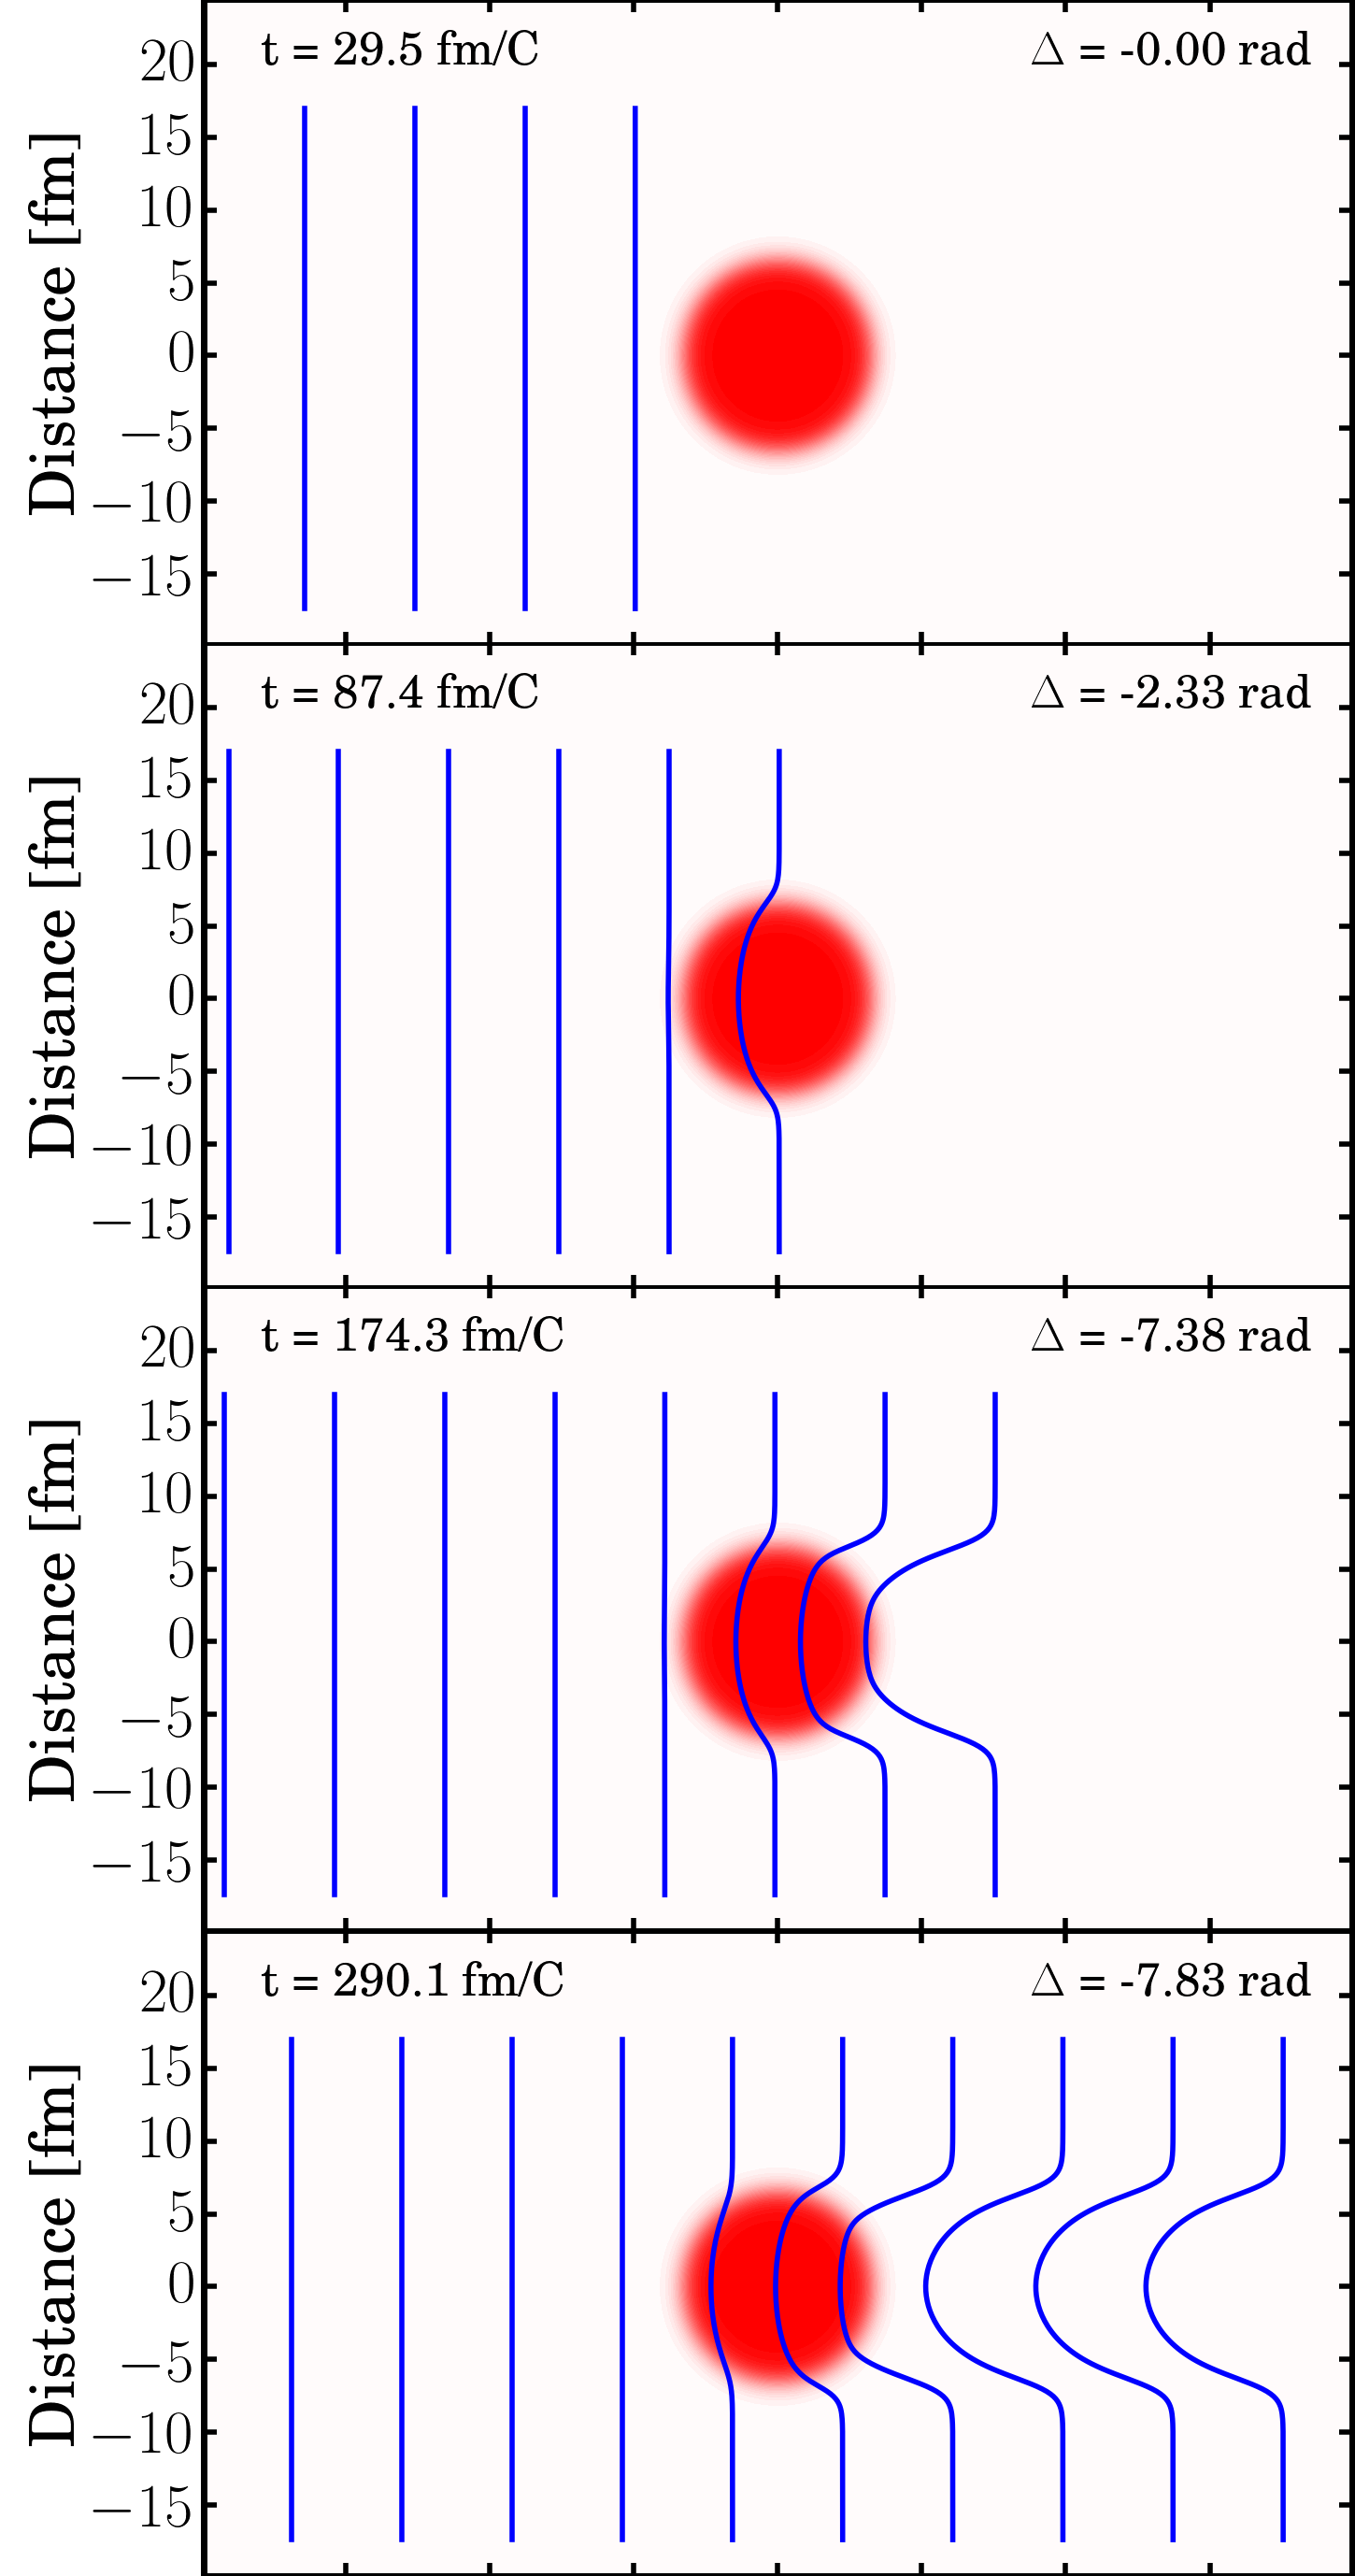
\includegraphics[width=0.5\textwidth]{figures/phaseShiftStillsFigure.png}
    \caption[A illustration of the nuclear Ramsauer effect]{
        A neutron wave train (series of
        blue lines) impinges from the left on a real Woods-Saxon
        potential centered at the origin (diffuse red circle). The potential
        refracts the neutron wave,
        retarding the phase of the wavefront as it passes through the
        potential. After escaping the potential, a phase difference $\Delta$ between
        the wave component passing \textit{around} and \textit{through the center}
        of the potential persists, resulting in scattering.
        For the leading wavefront in the wave train, $\Delta$ is indicated in
        the top right-hand corner of each panel. A differential version of
        Eq. \ref{phaseShift} is used to
        calculate the phase shift for each step. In this figure, the neutron
        energy $E_{n}$ = 14 MeV and nuclear mass $A$ = 25. For the Woods-Saxon potential,
        we used a potential depth $U$ = 42.8 MeV (following Angeli's analysis
        of \tot\ data at 14 MeV \cite{Angeli1970}), with nuclear radius $R = 
        r_{0}A^{\frac{1}{3}}$, $r_{0}$ = 1.4 fm, and a diffuseness parameter
        $a$ of 0.5 fm.
    }
    \label{RamsauerPhaseShiftFigure}
\end{figure}

Global OMs have been developed to simultaneously reproduce single nucleon, heavy ion,
and other hadron scattering data on targets across the chart of nuclides up to several
hundred MeV \cite{CH89, KoningDelaroche}. Because the proton-proton,
proton-neutron, and neutron-neutron scattering cross sections
are not identical, OM potentials are expected to differ for protons and
neutrons. Isoscalar terms, which respect isospin symmetry and thus treat protons and neutrons 
identically, account for most of the observed scattering data but do not include
any isospin-symmetry-breaking interactions known to exist between
nucleons, such as charged pion exchange. Thus isovector and isotensor terms,
which depend on the difference between the proton and neutron density
distributions in the nucleus, are needed. Constraining these terms requires data
on asymmetric nuclei, preferably highly-asymmetric nuclei, where the imbalance
of protons and neutrons makes any isovector effects most visible.

Despite their excellent reproduction of experiment, OMs involve the interaction of
many sometimes-opaque parameters with many incident
partial waves, complicating intuitive understanding of the underlying physics at work.
OMs are unabashedly phenomenogical so a wide variety of
experimental data types and energies are required to constrain the potential.
Where data are absent, model predictions are poor. A long-standing issue has
been a poor understanding of the isovector dependence of the real and
imaginary parts of optical potentials \cite{Holt16}, partially due to the
difficulty of neutron scattering experiments. As experimental facilities like
the Facility for Radioactive Isotope Beams (FRIB) come online and produce
extremely asymmetric nuclei, knowing the asymmetry-dependence of optical
potentials becomes paramount. Providing such experimental constraints for optical
potentials, in particular for the Dispersive Optical Model (DOM), is a primary 
motivation for the isotopically-resolved neutron \tot\ and \el\ work presented in this 
dissertation. In chapter \ref{DOMFormalism}, I present an overview of the DOM, a descendent of 
traditional OMs that extends the potential to the negative-energy domain, treating
nuclear structure and reactions on equal footing. 

%"The magnitude and energy dependence of the real isovector part of the
%optical potential are poorly constrained by experiment." \cite{Holt16}

Other topics that could be included:\\
- Hodgson's optical model review in 1971\\
- Microscopic OMs (folds interaction over nucleon density)\\
- Phenomenological OMs (no folding - use bulk)\\
- can largely follow Bob and Wim's review paper\\
- first formulated in 1949 to describe neutron cross section data\\
- separate proton and neutron global optical potentials in the 60s (Becchetti
and Greenlees)\\
- CH89 includes additional neutron scattering data on isotopic targets\\
- Lane potential \\
- Isovector versus isoscalar. Charged pion exchange mediates the isovector forces;
other nucleon-nucleon interactions mediate the isoscalar forces.

\section{Relevant Experimental Nuclear Data}

\subsection{Nucleon scattering data}
Elastic nucleon scattering cross sections, especially with protons, comprise the most extensively-measured
sector of experimental scattering databases. The EXFOR experimental reaction database
\cite{EXFORDatabase} contains thousands of proton and neutron
differential elastic scattering and analyzing
power data sets between 1-300 MeV, the domain relevant for this work. Optical model fits
to these data, both regional and global \cite{CH89, KoningDelaroche}, have helped
constrain nuclear radii \cite{radiusExample}, the strength of the spin-orbit coupling,
and revealed the importance of an imaginary spin-orbit term.

Inelastic nucleon scattering data is more difficult to collect experimentally and much sparser in
the literature record. By helping fix the strength and energy-dependence of the absorptive component
of the nuclear potential, inelastic data serve a complementary role to elastic
data. As was pointed out by Finlay et al. in 1993:

\begin{displayquote}
    "Above about 200 MeV, an impulse approximation might be expected to
    give a good description of the data, while at lower energy Pauli blocking and
    medium effects must be included. Phenomenologically, the imaginary term in
    the optical potential increases rapidly, while the real term is thought to
    pass through zero \cite{Finlay1993}."
\end{displayquote}

Isotopically-resolved data is particularly valuable for constraining nuclear
models, as it avoids averaging over multiple isotopes naturally present in many elemental samples.
Unfortunately, many pure isotopes are extremely expensive ($>$\$10,000 per gram) to
separate, putting them out of reach for all but the most well-funded experiments.
Indeed, as late as 1988, only a handful of neutron \tot\ measurement campaigns
on multiple samples had been conducted, most of them elemental, not isotopic
\cite{BarnBook1988}.

Figs. \ref{TCSChart} and \ref{RCSChart} illustrate the status of isotopically-resolved inelastic
nucleon scattering data in the EXFOR nuclear reaction database as of 2019.
Except for light isotopes and a few security-related actinides, coverage is
sparse and has changed little since the early 2000s. Isotopic proton \rxn\ measurements over
a broad energy range are particularly lacking due to the paucity of suitable
accelerators and the subtlety of the measurement. 
Both high-energy ($>$100 MeV) neutron \tot\ and proton \rxn\ data are essential for
understanding the asymmetry-dependence of the imaginary strength of the nuclear potential.
In this work, we focus on isotopically-resolved neutron scattering, which
is easier to measure and, when combined with proton \textit{elastic} cross sections,
provides information on the asymmetry-dependence of the real part of the nuclear potential.

\begin{sidewaysfigure}
    \centering
    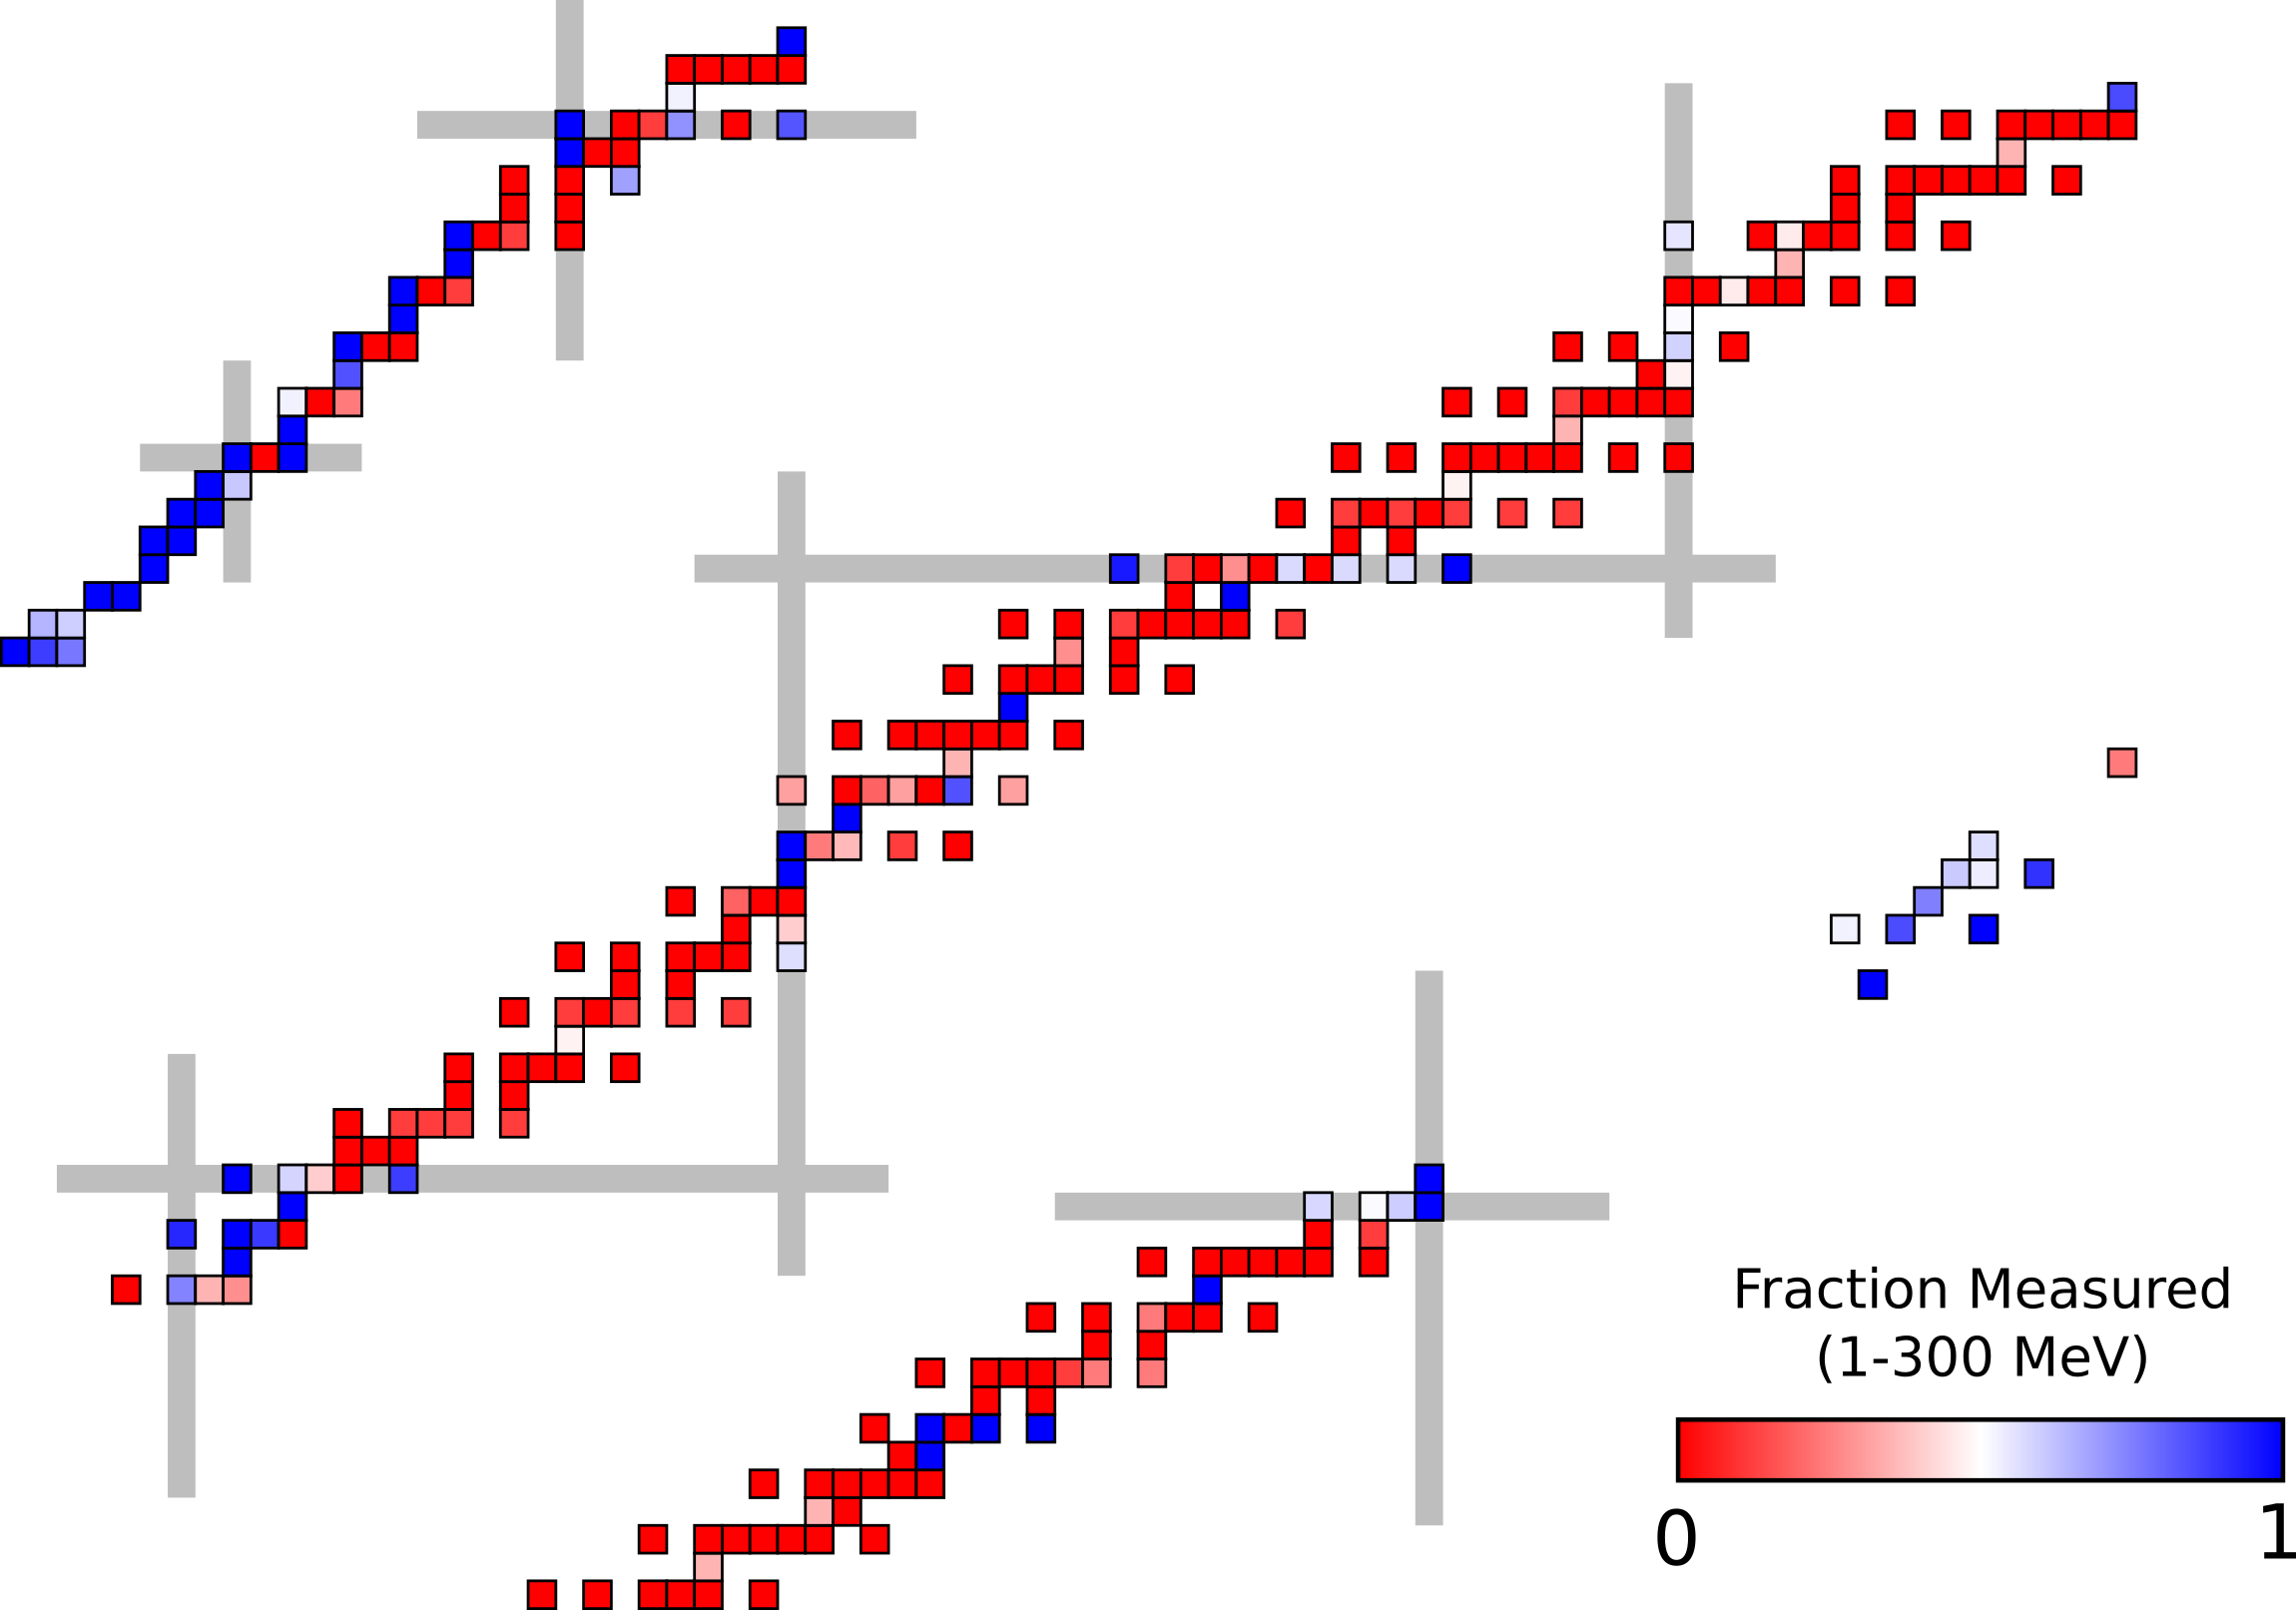
\includegraphics[width=0.9\textwidth]{figures/TCSChart.png}
    \caption[Landscape of existing neutron \tot\ data in 2019]
    {Isotopes are color-coded by the amount of neutron \tot\ data available in the EXFOR nuclear
        reaction database from 1-300 MeV, as accessed in 2018 and 2019. If data exists thoughout the
        1-300 MeV range, the isotope
        is colored blue. If no data exists, the isotope is colored red. For
        isotopes with partial coverage in this range, color varies by the degree
        of coverage. Except for the lightest
        isotopes (O and below), a few security-related actinides, there is almost no coverage
        throughout the nuclear chart. Our newly-measured results on \oSixEight, \niEightFour,
        \rhThree, and \snTwelveFour\ are included, as are a previous experiment on
        \caAughtEight \cite{Shane2010}.
    }
    \label{TCSChart}
\end{sidewaysfigure}

\begin{sidewaysfigure}
    \centering
    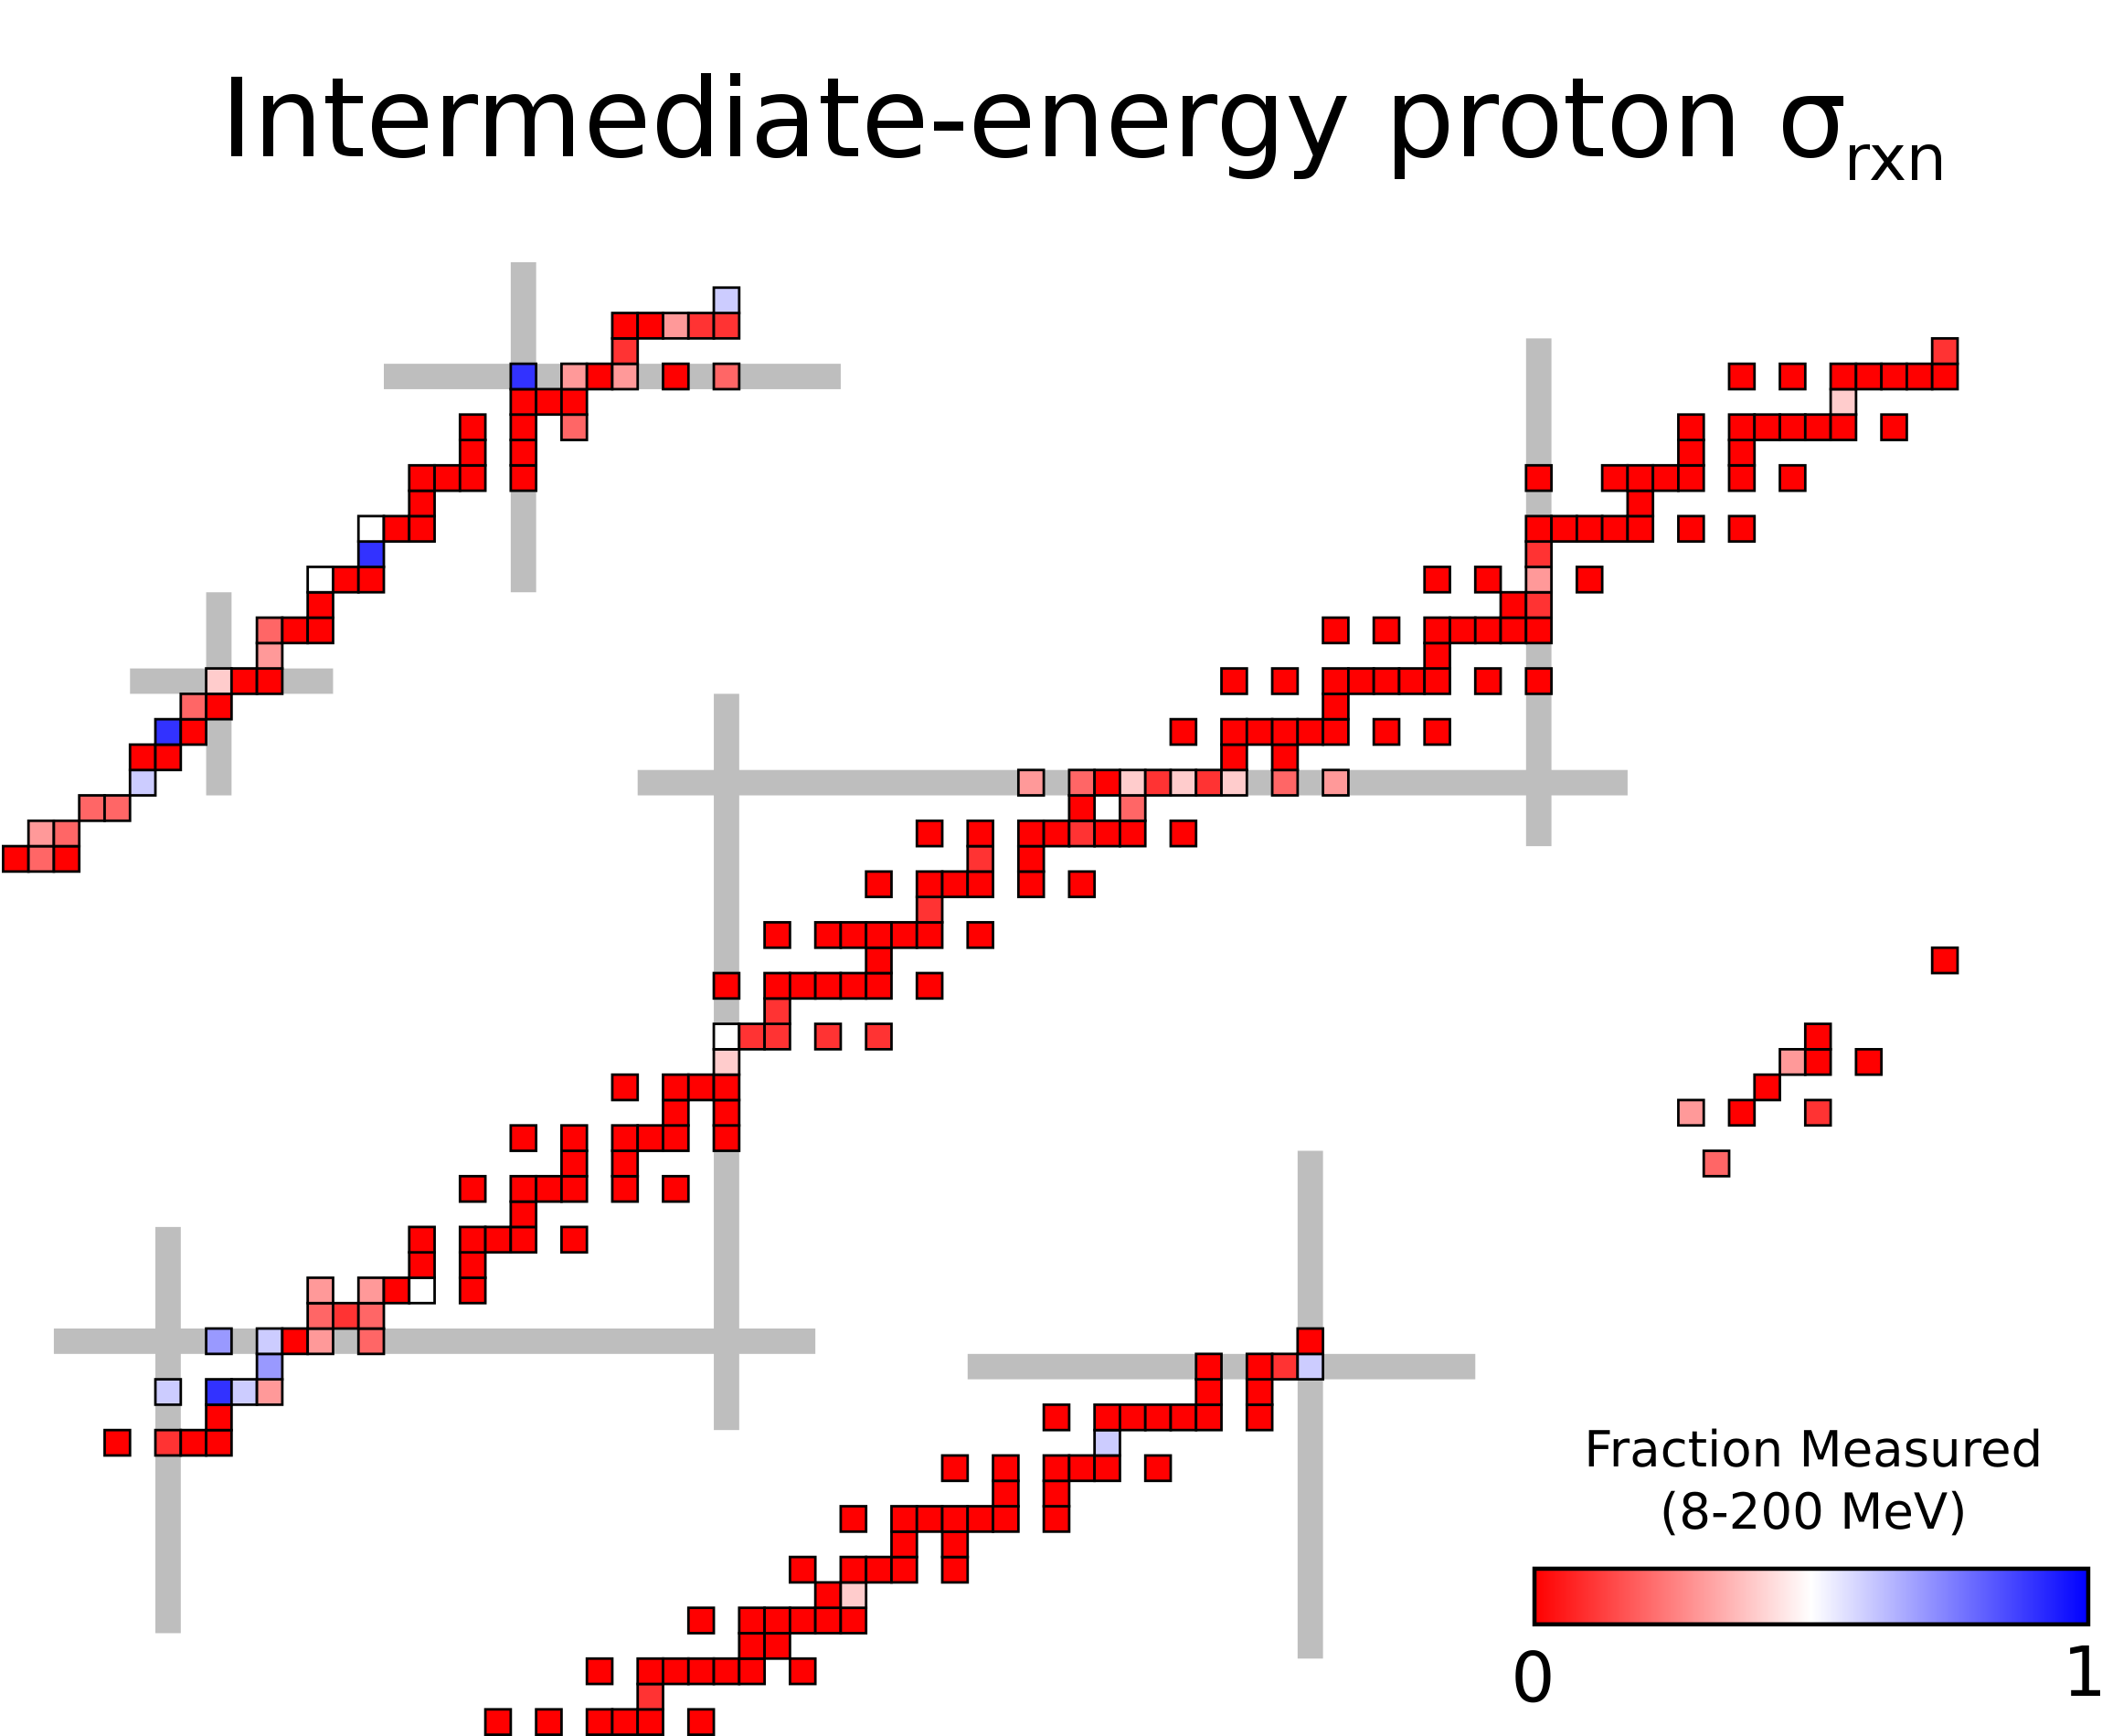
\includegraphics[width=0.9\textwidth]{figures/RCSChart.png}
    \caption[Landscape of existing proton \rxn\ data in 2019]
    {Isotopes are color-coded by the amount of neutron \tot\ data available in the EXFOR nuclear
        reaction database from 1-300 MeV, as accessed in 2018 and 2019. If data exists thoughout the 1-300 MeV range, the isotope
        is colored blue. If no data exists, the isotope is colored red. For
        isotopes with partial coverage in this range, color varies by the degree
        of coverage. Almost no nuclei have experimental coverage throughout this energy
        range, a testament to the difficulty of proton \rxn\ measurements.}
    \label{RCSChart}
\end{sidewaysfigure}

\subsection{Quasi-free scattering data: (e,e'p), (p,2p), and (p,pn)}
Louk Lapikas
NIKHEF data on 16O, 40Ca, 208Pb
SRCs and LRCs

\subsection{Nuclear Masses, Matter Radii, and Charge Radii}
Connect to Vinas, Chuck Horowitz, and J. Piekarewicz's neutron star EOS work.
neutron skin first mention: \cite{Wilkinson1967}
HF-BCS treatment of 700 nuclei to calculate proton and neutron RMS radii \cite{Angeli1980}

Electron scattering and laser spectroscopy
K. Minamisono

\section{Motivation, Scope, and Dissertation Outline}
Improved isotopically-resolved neutron scattering data are an essential ingredient
for better nuclear reaction models and to test the asymmetry-dependence of the
nuclear potential. The results of our campaign to produce these valuable
\tot\ and \el\ data sets on cornerstone nuclei form the backbone of this dissertation.
In addition to these experimental results, a suite of Dispersive Optical Model (DOM) analyses that 
incorporate these new data is presented. From the DOM potentials, a variety of asymmetry-dependent 
nuclear-structure quantities, including neutron skins and relative momentum
content, are extracted.

An overview of neutron \tot\ experimental considerations, the details of our 
\tot\ experiment, and analysis for our isotopically-resolved \tot\ measurements
on \oSixEight, \niEightFour, \rhThree, and \snTwelveFour\ are detailed in 
Chapters \ref{TCSExperiment} and \ref{TCSAnalysis}. Similarly, our elastic scattering measurements 
on \snTwelveFour\ are presented in Chapters \ref{ECSExperiment} and \ref{ECSAnalysis}. A brief 
summary of the Dispersive Optical Model formalism is
given in Chapter \ref{DOMFormalism} and the results from our DOM fits of \oSixEight, 
\caAughtEight, \niEightFour, \snTwelveFour, and \pbEight\ are presented in Chapter \ref{DOMResults}. 
A complete listing of the experimental data used in the DOM analyses, the
parameter values of the DOM potentials, and figures showing the 
results of the DOM fits are provided in Appendices \ref{DOMDataSets},
\ref{DOMParameters}, and \ref{DOMFits}. 
